\documentclass[10pt]{article}
\usepackage[polish]{babel}
\usepackage[utf8]{inputenc}
\usepackage[T1]{fontenc}
\usepackage{amsmath}
\usepackage{amsfonts}
\usepackage{amssymb}
\usepackage[version=4]{mhchem}
\usepackage{stmaryrd}
\usepackage{graphicx}
\usepackage[export]{adjustbox}
\graphicspath{ {./images/} }
\usepackage{hyperref}
\hypersetup{colorlinks=true, linkcolor=blue, filecolor=magenta, urlcolor=cyan,}
\urlstyle{same}

\title{GIMNAZJUM }

\author{}
\date{}


%New command to display footnote whose markers will always be hidden
\let\svthefootnote\thefootnote
\newcommand\blfootnotetext[1]{%
  \let\thefootnote\relax\footnote{#1}%
  \addtocounter{footnote}{-1}%
  \let\thefootnote\svthefootnote%
}

%Overriding the \footnotetext command to hide the marker if its value is `0`
\let\svfootnotetext\footnotetext
\renewcommand\footnotetext[2][?]{%
  \if\relax#1\relax%
    \ifnum\value{footnote}=0\blfootnotetext{#2}\else\svfootnotetext{#2}\fi%
  \else%
    \if?#1\ifnum\value{footnote}=0\blfootnotetext{#2}\else\svfootnotetext{#2}\fi%
    \else\svfootnotetext[#1]{#2}\fi%
  \fi
}

\begin{document}
\maketitle
\begin{enumerate}
  \item Oblicz różnicę:
\end{enumerate}

\[
\left(1^{2}+2^{2}+3^{2}+\cdots+2016^{2}\right)-(1 \cdot 3+2 \cdot 4+3 \cdot 5+\cdots+2015 \cdot 2017)
\]

\begin{enumerate}
  \setcounter{enumi}{1}
  \item Ile liczb trzycyfrowych podzielnych przez 9 ma następującą własność: suma cyfr ilorazu tej liczby przez 9 jest o 9 mniejsza od sumy jej cyfr?
  \item Rysunek obok przedstawia kwadratową płytkę. Narysowane na niej linie krzywe są ćwiartkami okręgów o promieniu równym połowie boku płytki. Długość takiej ćwiartki jest równa 5 dm. Z 16 takich płytek budujemy kwadrat. Jaką maksymalną długość może mieć nieprzerwana linia utworzona z tych ćwiartek okręgów?\\
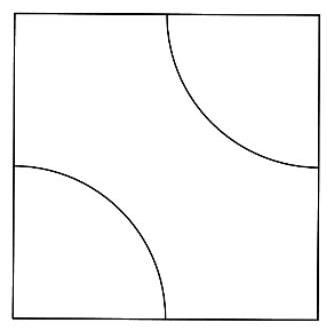
\includegraphics[max width=\textwidth, center]{2024_11_21_1dc4d69aa02a10172350g-1}
\end{enumerate}

\section*{LICEUM}
\begin{enumerate}
  \item W szkolnym turnieju piłki ręcznej każda drużyna rozegrała z każdą inną dokładnie jeden mecz. Drużyna zwycięska zdobywała 2 punkty, przegrana 0 punktów, w przypadku zaś remisu obie drużyny otrzymywały po jednym punkcie. Zwycięzca turnieju zdobył w czasie całych rozgrywek 7 punktów, drużyna druga 5 punktów, a drużyna trzecia 3 punkty. Ile punktów zdobyła drużyna, która zajęła ostatnie miejsce?
  \item Funkcja \(f\) określona jest na zbiorze liczb naturalnych wzorem
\end{enumerate}

\[
f(n)=\left\{\begin{array}{cc}
n+5 & \text { gdy } n \text { jest liczbą nieparzystą } \\
\frac{n}{2} & \text { gdy } n \text { jest liczbą parzystą }
\end{array}\right.
\]

Ile jest równa suma cyfr liczby nieparzystej \(k\), dla której \(f(f(f(k)))=35\) ?\\
3. Ile co najwyżej trójelementowych podzbiorów można utworzyć z elementów zbioru siedmioelementowego w taki sposób, aby każde dwa z powstałych podzbiorów miały dokładnie jeden element wspólny?

\footnotetext{Rozwiqzania należy oddać do piatku 5 lutego do godziny 10.35 koordynatorowi konkursu panu Jarostawowi Szczepaniakowi lub swojemu nauczycielowi matematyki lub przestać na adres \href{mailto:jareksz@interia.pl}{jareksz@interia.pl} do piatku 5 lutego do pótnocy.
}
\end{document}